\documentclass[12pt]{report}
\usepackage[a4paper]{geometry}
\usepackage[myheadings]{fullpage}
\usepackage{fancyhdr}
\usepackage{lastpage}
\usepackage{graphicx, wrapfig, subcaption, setspace, booktabs}
\usepackage[T1]{fontenc}
\usepackage[font=small, labelfont=bf]{caption}
\usepackage{fourier}
 \usepackage{listings}
\graphicspath{ {Azure_StreamAnalytics-Kotti-Nampouri/config_screenshots/} }
\usepackage[english]{babel}
\usepackage{sectsty}
\usepackage{url, lipsum}
\usepackage{tgbonum}
\usepackage{xcolor}
\usepackage[none]{hyphenat}
\usepackage[bottom]{footmisc}
\usepackage{float}



\sloppy
% Handle 'Underfull \hbox or \vbox' warnings
\usepackage{etoolbox}
\apptocmd{\sloppy}{\hbadness 10000\relax}{}{}
\apptocmd{\sloppy}{\vbadness 10000\relax}{}{}
% Add date
\usepackage[useregional]{datetime2}
\newcommand{\mydate}{\DTMdisplaydate{2019}{7}{5}{-1}}
% Change Content numbering
\renewcommand{\thesection}{\arabic{section}}
\renewcommand{\labelitemi}{\tiny$\blacksquare$}
% Packages for Python code
\usepackage{listings}
\usepackage{color}
\usepackage[colorlinks]{hyperref} 
\definecolor{codegreen}{rgb}{0,0.6,0}
\definecolor{codegray}{rgb}{0.5,0.5,0.5}
\definecolor{codepurple}{rgb}{0.58,0,0.82}
\definecolor{backcolour}{rgb}{0.95,0.95,0.92}
 
\lstdefinestyle{mystyle}{
    backgroundcolor=\color{backcolour},   
    commentstyle=\color{codegreen},
    keywordstyle=\color{magenta},
    numberstyle=\tiny\color{codegray},
    string=[s]{"}{"},
    stringstyle=\color{blue},
    comment=[l]{:},
    basicstyle=\footnotesize,
    breakatwhitespace=false,         
    breaklines=true,                 
    captionpos=b,                    
    keepspaces=true,                 
    numbers=left,                    
    numbersep=5pt,                  
    showspaces=false,                
    showstringspaces=false,
    showtabs=false,                  
    tabsize=2
}
 
\lstset{style=mystyle}

\newcommand{\HRule}[1]{\rule{\linewidth}{#1}}
\onehalfspacing
\setcounter{tocdepth}{5}
\setcounter{secnumdepth}{5}

\begin{document}
{\fontfamily{cmr}\selectfont
\title{ \normalsize \textsc{}
		\\ [2.0cm]
		\HRule{0.5pt} \\
		\LARGE \textbf{\uppercase{Big Data Management Systems:\\
		PROJECT \#4 --
		AZURE STREAM ANALYTICS}
		\HRule{2pt} \\ [0.5cm]
		\normalsize \mydate \vspace*{5\baselineskip}}
		}
\date{}

\author{
		Zoe Kotti and Chryssa Nampouri \\ 
		\textit{Department of Management Science and Technology} \\
		\textit{Athens University of Economics and Business} \\
		Athens, Greece \\
		\{t8150062, t8150096\}@aueb.gr \\
		\\
		Supervisor: Prof. Damianos Chatziantoniou
}

\maketitle
\tableofcontents
\newpage

\sectionfont{\scshape}

\section{Project Description}
In the context of this assignment a set of Reference Data is given that consists of three JSON files:

\begin{enumerate}
\item \textbf{Customer.json:} Personal data about customers who have made transactions. Each customer example is described by the following attributes: 
	\begin{itemize}
	\item \textit{card\_number} (integer) 
	\item \textit{first\_name} (string)
	\item \textit{last\_name} (string)
	\item \textit{age} (integer)
	\item \textit{gender} (string)
	\item \textit{area\_code} (integer)
	\end{itemize}
\item \textbf{Atm.json:} Describes ATMs as:
	\begin{itemize}
	\item \textit{atm\_code} (integer)
	\item \textit{area\_code} (integer)
	\end{itemize}
\item \textbf{Area.json:} Describes areas as:
	\begin{itemize}
	\item \textit{area\_code} (integer)
	\item \textit{area\_country} (string)
	\item \textit{area\_city} (string)
	\end{itemize}
\end{enumerate}

\noindent The purpose of this project was to process a data stream of ATM transactions and answer stream queries. The schema of the stream is the following: (ATMCode, CardNumber, Type, Amount).

\newpage

\section{Azure Configuration}
In order to execute the above process on Azure Stream Analytics Platform the following steps are required:
\begin{enumerate}
    	\item Create an Azure account.
        \item Setup an Event Hub.
        \item Generate a Security Access Signature \footnote{\url{https://github.com/sandrinodimattia/RedDog/releases }}.
        \item Edit Generator.html and update the CONFIG variables with your security access signature.
        \item Feed the Event Hub with streaming data by using the 				Generator.html.
        \item Setup a Storage account.
        \item Upload the Reference Data files to your storage account.
        \item Setup a Stream Analytics Job.
        \item Use the Event Hub and the Reference Data Files as Input.
        \item Create a Blob Storage Output.
        \item Run queries.

\end{enumerate}
\newpage

\section{Azure Configuration: Screenshots}

\begin{figure}[H]
	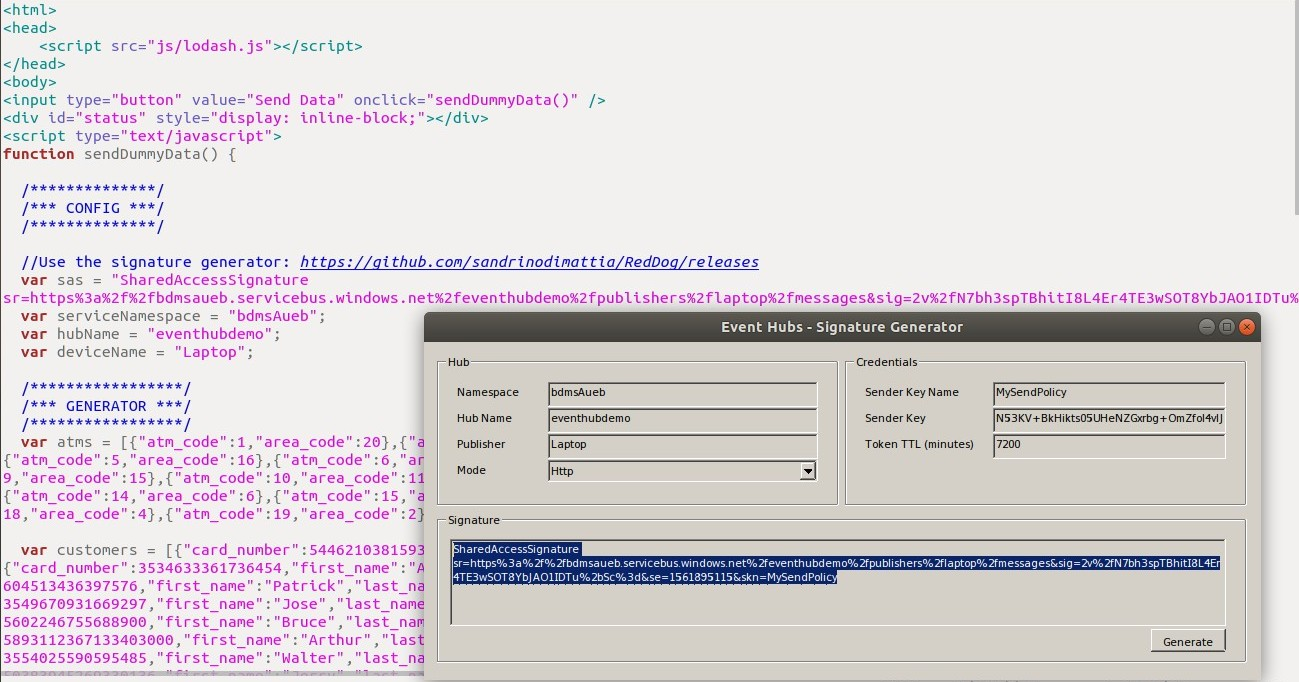
\includegraphics[width=\textwidth]{config_generator.jpg}
	\caption{Security Access Signature (\textit{Step 3,4).}}
\end{figure}

\begin{figure}[H]
	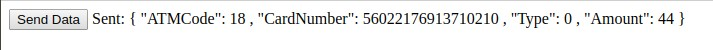
\includegraphics[width=\textwidth]{generator.jpg}
	\caption{Random Data Generator (\textit{Step 5).}}
\end{figure}


\begin{figure}[H]
	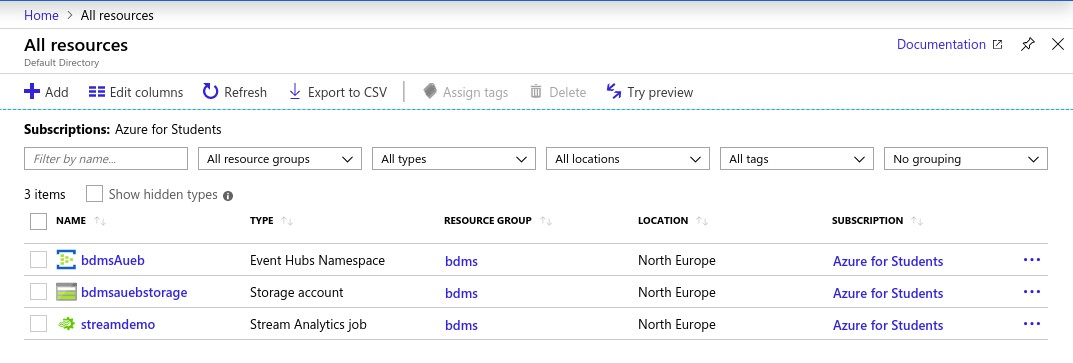
\includegraphics[width=\textwidth]{all_resources.jpg}
	\caption{All Resources (\textit{Step 2, 6, 8).}}
\end{figure}

\begin{figure}[H]
	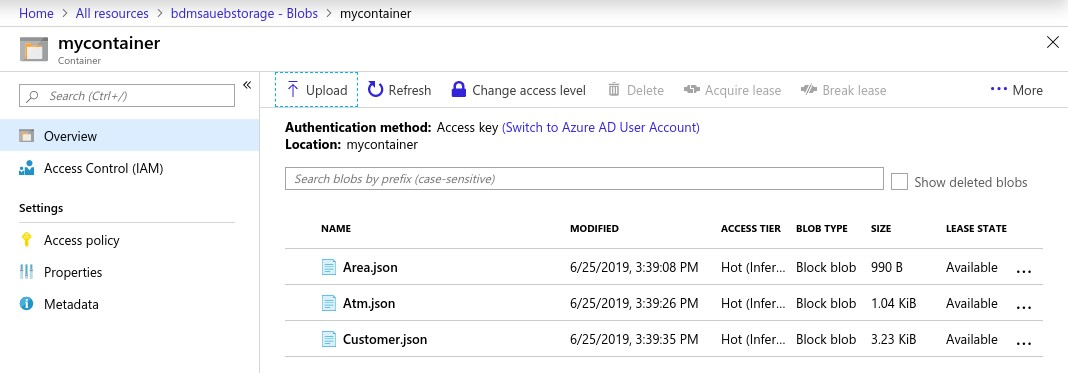
\includegraphics[width=\textwidth]{upload_reference_data.jpg}
	\caption{Storage Account (\textit{Step 7).}}
\end{figure}

\begin{figure}[H]
	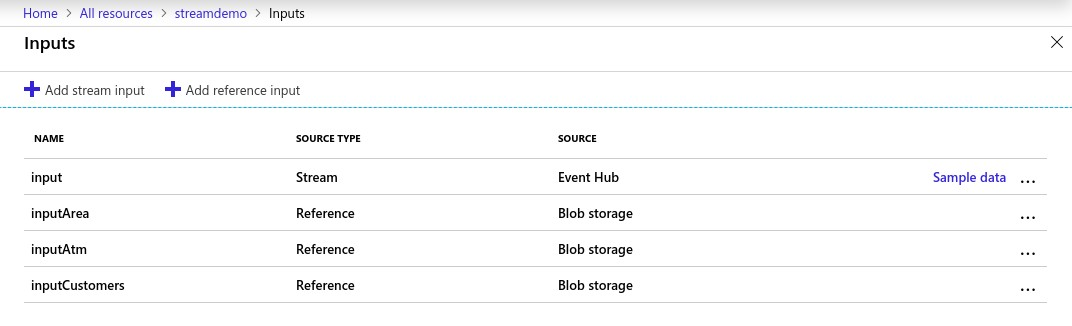
\includegraphics[width=\textwidth]{job_inputs.jpg}
	\caption{Job Inputs (\textit{Step 9).}}
\end{figure}

\begin{figure}[H]
	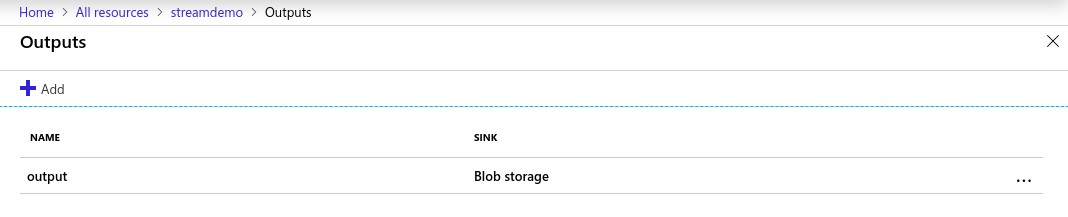
\includegraphics[width=\textwidth]{output.jpg}
	\caption{Job Output (\textit{Step 10).}}
\end{figure}

\newpage

\section{Azure Stream Analytics: Queries}

After specifying the input source of the streaming data and the output sink for the results, the following queries were expressed in a \textit{ SQL-like query language (T-SQL)}, in order to be executed on the Azure Platform:

\begin{enumerate}
\item Show the total 'Amount' of 'Type = 0' transactions at 'ATM Code = 21' of the last 10 minutes. Repeat as new events keep flowing in (use a sliding window).
\item Show the total 'Amount' of 'Type = 1' transactions at 'ATM Code = 21' of the last hour. Repeat once every hour (use a tumbling window).
\item Show the total 'Amount' of 'Type = 1' transactions at 'ATM Code = 21' of the last hour. Repeat once every 30 minutes (use a hopping window).
\item Show the total 'Amount' of 'Type = 1' transactions per 'ATM Code' of the last one hour (use a sliding window).
\item Show the total 'Amount' of 'Type = 1' transactions per 'Area Code' of the last hour. Repeat once every hour (use a tumbling window).
\item Show the total 'Amount' per ATM's 'City' and Customer's 'Gender' of the last hour. Repeat once every hour (use a tumbling window).
\item Alert (SELECT '1') if a Customer has performed two transactions of 'Type = 1' in a window of an hour (use a sliding window).
\item Alert (SELECT '1') if the 'Area Code' of the ATM of the transaction is not the same as the 'Area Code' of the 'Card Number' (Customer's Area Code) - (use a sliding window)
\end{enumerate}

\noindent For each of the above queries we ran a stream analytics job and we present some indicative results in the report below. In some cases, we reduced the time limit of the windows, in order to precipitate the progress of the data transformation. 

\newpage

\textbf{Query 1:}


\begin{lstlisting} [language=SQL]
/*
    Q1: Show the total 'Amount' of 'Type = 0' transactions at
    'ATM Code = 21' of the last 10 minutes. Repeat as new events keep
    flowing in (use a sliding window).
*/

SELECT
    sum(CAST([input].[Amount] AS BIGINT)) as Total_Amount, 
    System.Timestamp() AS Event_Time
INTO [output]
FROM [input]
WHERE [input].[Type] = 0 and [input].[ATMCode] = 21
GROUP BY SlidingWindow(minute, 10)

\end{lstlisting}

\bigbreak

\noindent \textbf{Output\_1 (SlidingWindow(second, 10)): }

\begin{lstlisting}
[
	{  
	   "Total_Amount":21,
	   "Event_Time":"2019-07-03T00:18:29.2580000Z"
	},
	{  
	   "Total_Amount":38,
	   "Event_Time":"2019-07-03T00:18:39.2430000Z"
	},
	{  
	   "Total_Amount":17,
	   "Event_Time":"2019-07-03T00:18:39.2580000Z"
	},
	{  
	   "Total_Amount":105,
	   "Event_Time":"2019-07-03T00:18:40.2430000Z"
	},
	{  
	   "Total_Amount":88,
	   "Event_Time":"2019-07-03T00:18:49.2430000Z"
	},
	{  
	   "Total_Amount":119,
	   "Event_Time":"2019-07-03T00:18:49.2590000Z"
	}
]
\end{lstlisting}


\noindent \textbf{Query 2:}
\begin{lstlisting} [language=SQL]
/*
    Q2: Show the total 'Amount' of 'Type = 1' transactions at 
    'ATM Code = 21' of the last hour. Repeat once every hour 
    (use a tumbling window).
*/

SELECT
    sum(CAST([input].[Amount] AS BIGINT)) as Total_Amount, 
    System.Timestamp() AS Time
INTO [output]
FROM [input]
WHERE [input].[Type] = 1 and [input].[ATMCode] = 21
GROUP BY TumblingWindow(hour, 1)

\end{lstlisting}
\bigbreak
\noindent \textbf{Output\_2 (TumblingWindow(minute, 1)): }
\begin{lstlisting}
[
	{
		"Total_Amount": 335,
		"Event_Time": "2019-06-29T17:36:00.0000000Z"
	},
	{
		"Total_Amount": 603,
		"Event_Time": "2019-06-29T17:37:00.0000000Z"
	},
	{
		"Total_Amount": 465,
		"Event_Time": "2019-06-29T17:38:00.0000000Z"
	}
]
\end{lstlisting}

\newpage
\noindent \textbf{Query 3:}

\begin{lstlisting} [language=SQL]
/*
    Q3: Show the total 'Amount' of 'Type = 1' transactions at 
    'ATM Code = 21' of the last hour. Repeat once every 30 minutes 
    (use a hopping window).
*/

SELECT
    sum(CAST([input].[Amount] AS BIGINT)) as Total_Amount, 
    System.Timestamp() AS Time
INTO [output]
FROM [input]
WHERE [input].[Type] = 1 and [input].[ATMCode] = 21
GROUP BY HoppingWindow(minute, 60, 30)


\end{lstlisting}
\bigbreak


\noindent \textbf{Output\_3 (HoppingWindow(second, 60, 30)): }
\begin{lstlisting}
[
	{
		"Total_Amount": 406,
		"Event_Time": "2019-06-29T17:48:00.0000000Z"
	},
	{
		"Total_Amount": 651,
		"Event_Time": "2019-06-29T17:48:30.0000000Z"
	},
	{
		"Total_Amount": 728,
		"Event_Time": "2019-06-29T17:49:00.0000000Z"
	}
]
\end{lstlisting}

\newpage
\noindent \textbf{Query 4:}

\begin{lstlisting} [language=SQL]
/*
    Q4: Show the total 'Amount' of 'Type = 1' transactions per 'ATM Code'
    of the last one hour (use a sliding window).
*/

SELECT
    [input].[ATMCode],
    sum(CAST([input].[Amount] AS BIGINT)) as Total_Amount, 
    System.Timestamp() AS Time
INTO [output]
FROM [input]
WHERE Type = 1
GROUP BY [input].[ATMCode],
         SlidingWindow(hour, 1)


\end{lstlisting}

\bigbreak


\noindent \textbf{Output\_4 (SlidingWindow(minute, 1)): }
\begin{lstlisting}
[
	{
		"ATMCode":15
		"Total_Amount": 2519,
		"Event_Time": "2019-06-29T17:56:55.2870000Z"
	},
	{
		"ATMCode":18
		"Total_Amount": 1624,
		"Event_Time": "2019-06-29T17:56:55.2920000Z"
	},
	{
		"ATMCode":18
		"Total_Amount": 1660,
		"Event_Time": "2019-06-29T17:56:55.3020000Z"
	},
	{
		"ATMCode":19
		"Total_Amount": 2031,
		"Event_Time": "2019-06-29T17:56:55.3020000Z"
	}
]
\end{lstlisting}


\newpage

\noindent \textbf{Query 5:}

\begin{lstlisting} [language=SQL]
/*
    Q5: Show the total 'Amount' of 'Type = 1' transactions per 'Area Code'
    of the last hour. Repeat once every hour (use a tumbling window).
*/

SELECT
    [inputAtm].[area_code],
    sum(CAST([input].[Amount] AS BIGINT)) as Total_Amount, 
    System.Timestamp() AS Time
INTO [output]
FROM [input]
INNER JOIN [inputAtm] 
    ON [input].[ATMCode] = [inputAtm].[atm_code] 
WHERE [input].[Type] = 1
GROUP BY [inputAtm].[area_code],
         TumblingWindow(hour, 1)


\end{lstlisting}

\bigbreak

\noindent \textbf{Output\_5 (TumblingWindow(minute, 1)): }
\begin{lstlisting}
[
	{  
	   "area_code":10,
	   "Total_Amount":670,
	   "Time":"2019-06-30T09:40:00.0000000Z"
	},
	{  
	   "area_code":14,
	   "Total_Amount":43,
	   "Time":"2019-06-30T09:40:00.0000000Z"
	},
	{  
	   "area_code":12,
	   "Total_Amount":50,
	   "Time":"2019-06-30T09:40:00.0000000Z"
	},
	{  
	   "area_code":2,
	   "Total_Amount":1813,
	   "Time":"2019-06-30T09:40:00.0000000Z"
	}
]
\end{lstlisting}


\noindent \textbf{Query 6:}

\begin{lstlisting} [language=SQL]
/*
    Q6: Show the total 'Amount' per ATM's 'City' and Customer's 'Gender' 
    of the last hour. Repeat once every hour (use a tumbling window).
*/

SELECT
    [inputArea].[area_city],
    [inputCustomers].[gender],
    sum(CAST([input].[Amount] AS BIGINT)) as Total_Amount, 
    System.Timestamp() AS Time
INTO [output]
FROM [input]
INNER JOIN [inputAtm]
    ON [input].[ATMCode] = [inputAtm].[atm_code] 
INNER JOIN [inputArea]
    ON [inputAtm].[area_code] = [inputArea].[area_code]
INNER JOIN [inputCustomers]
    ON [input].[CardNumber] = [inputCustomers].[card_number]
GROUP BY [inputArea].[area_city],
         [inputCustomers].[gender], 
         TumblingWindow(hour, 1)

\end{lstlisting}
\bigbreak

\noindent \textbf{Output\_6 (TumblingWindow(minute, 1)):}
\begin{lstlisting}
[
	{  
	   "area_city":"Springfield",
	   "gender":"Male",
	   "Total_Amount":1066,
	   "Time":"2019-06-30T20:12:00.0000000Z"
	},
	{  
	   "area_city":"Baltimore",
	   "gender":"Male",
	   "Total_Amount":384,
	   "Time":"2019-06-30T20:12:00.0000000Z"
	}
]
\end{lstlisting}

\newpage
\noindent \textbf{Query 7:}

\begin{lstlisting} [language=SQL]
/*
    Q7: Alert (SELECT '1') if a Customer has performed two transactions
    of 'Type = 1' in a window of an hour (use a sliding window).
*/

SELECT
    [inputCustomers].[first_name],
    [inputCustomers].[last_name],
    [input].[CardNumber] AS Card_Number,
    COUNT (*) AS Transactions,
    System.Timestamp AS Time
INTO [output]
FROM [input]
INNER JOIN [inputCustomers]
    ON [inputCustomers].[card_number] = [input].[CardNumber]
WHERE [input].[Type] = 1
GROUP BY [inputCustomers].[first_name],
         [inputCustomers].[last_name],
         [input].[CardNumber],
         SlidingWindow(hour, 1)
HAVING Transactions = 2

\end{lstlisting}

\bigbreak

\noindent \textbf{Output\_7 (SlidingWindow(hour, 1)): }
\begin{lstlisting}
[
	{  
	   "first_name":"Brenda",
	   "last_name":"Carroll",
	   "Card_Number":560222217915598000,
	   "Transactions":2,
	   "Time":"2019-06-30T12:49:59.7440000Z"
	},
	{  
	   "first_name":"Bruce",
	   "last_name":"Morrison",
	   "Card_Number":5602246755688900,
	   "Transactions":2,
	   "Time":"2019-06-30T12:50:02.6970000Z"
	}
]
\end{lstlisting}
\newpage

\noindent \textbf{Query 8:}

\begin{lstlisting} [language=SQL]
/*
    Q8: Alert (SELECT '1') if the 'Area Code' of the ATM of the transaction 
    is not the same as the 'Area Code' of the 'Card Number' 
    (Customer's Area Code) - (use a sliding window).
*/

SELECT
    [inputAtm].[area_code] AS Atm_Area_Code,
    [inputCustomers].[area_code] AS Customer_Area_Code,
    COUNT (*),
    System.Timestamp AS Time
INTO [output]
FROM [input]
INNER JOIN [inputCustomers]
    ON [inputCustomers].[card_number] = [input].[CardNumber]
INNER JOIN [inputAtm]
    ON [inputAtm].[atm_code] = [input].[ATMCode]
WHERE [inputAtm].[area_code] != [inputCustomers].[area_code]
GROUP BY [inputAtm].[area_code],
         [inputCustomers].[area_code], 
         SlidingWindow(hour, 1)

\end{lstlisting}

\bigbreak

\noindent \textbf{Output\_8 (SlidingWindow(hour, 1)): }
\begin{lstlisting}
[
	{  
	   "Atm_Area_Code":5,
	   "Customer_Area_Code":7,
	   "COUNT":523,
	   "Time":"2019-06-30T20:18:13.5610000Z"
	},
	{  
	   "Atm_Area_Code":2,
	   "Customer_Area_Code":1,
	   "COUNT":333,
	   "Time":"2019-06-30T20:18:13.5760000Z"
	}
]
\end{lstlisting}

\newpage
\nocite{*}
\bibliography{report}
\underline{}
\bibliographystyle{ieeetr}

\end{document}